\section{Mathematic Model}
In this part, we describe the minimum surfaces and obstacles problems in Section 2.1 and formulate them mathematically in Section 2.2.
\subsection{Model Description}
\subsubsection{Minimum Surfaces}
The minimum surface problem is to generate a two dimensional surface that is defined on a set $\Omega \subset \mathbb{R}^{2}$ only from data and observations given at the boundary of $\Omega.$ In particular, let $\Gamma=\partial \Omega$ denote the boundary of the set $\Omega$ and let $r: \Gamma \rightarrow \mathbb{R}$ be a given function on $\Gamma .$ Then, we will solve a discretized, finite-dimensional minimization task to find a function $q: \operatorname{cl} \Omega \rightarrow \mathbb{R}$ satisfying the following goals:

\begin{itemize}
    \item $ q(t)=r(t) \quad \forall t \in \Gamma$.
    \item The graph of $q$ has minimum surface.
\end{itemize}
\subsubsection{Obstacle Problems}
The minimum surface problem could be further extended into obstacle problems, which means the reference set $\Omega$ contains additional obstacles that need to be considered when building the function $q$. As shown previously, the boundary set $\Gamma=\partial \Omega$ and boundary function $r: \Gamma \rightarrow \mathbb{R}$ are the same as minimum surface problem. Moreover, let $\mathcal{B} \subset \Omega$ be an obstacle set and let $b: \mathcal{B} \rightarrow \mathbb{R}$ be a given obstacle function. Here, we will utilize different approaches to solve the constrained problem under different types of obstacles, to find a function $q: \operatorname{cl} \Omega \rightarrow \mathbb{R}$ satisfying the following goals:
\begin{itemize}
  \item $ q(t)=r(t) \quad \forall t \in \Gamma$. 
  \item $ q(t) \geq b(t) \quad \forall t \in \mathcal{B} $.
  \item The graph of $q$ has minimum surface.
\end{itemize}



\subsection{Model Formulation}
The process of solving the original problem is acutually finding an optimal solution in a function space, that is, we are trying to find $f: R^3 \rightarrow 0 $. If we find such function in a function space, we need to utilize $f_{x,y,z} = \mathop{\arg\min}_{f} \iint_{S} f(x,y,z) ds$, where $x,y,z \in R$ and $z=z(x,y)$. There are some constraints described above. This is a very hard process since the space we are searching in is the \textbf{function space} rather than the \textbf{numerical space}. In order to simplify the solving process, we can use the technique of \textbf{parameterization}. This is acutually a \textbf{generalized explanation} for the \textbf{discretization approach} given by the project requirement.

One common way to parameterization is to discretize the surface. We can use gridding to discretize the the input of $z_{x,y}$, that is, we use $(i,j) \in \mathbb{Z} \times \mathbb{Z}$ to represent $(x,y) \in \mathbb{R} \times \mathbb{R}$ and use parameter $\theta_{i,j}$ to represent the surface $f_{x,y,z}$. Correspondingly, the area $\iint_{S} f(x,y,z) ds$ can be represent as the area of rectangles in the $R^3$ space by rectangular tessellation or that of triangles by triangular tessellation. An example of triangular tessellation is shown on Figure \ref{fig:discretization}.

\begin{figure}[!htbp]
    \centering
      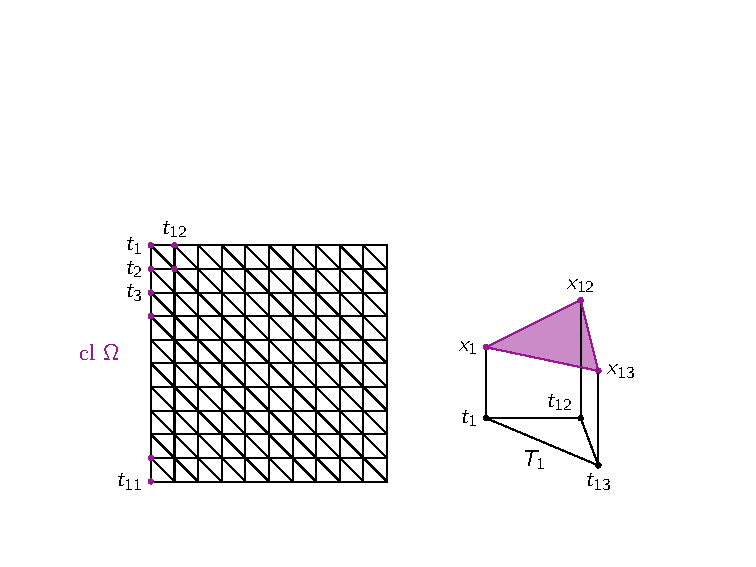
\includegraphics[width=10cm]{images/discretization.pdf}
      \caption{An Example of Parameterization by Discretization \\ (Copied from CIE6010 Lecture 1, by Prof. Andre Milzarek)}
      \label{fig:discretization}
\end{figure}

We can see that if we switch $\theta_{i,j}$ to $x_{i,j}$, we will exactly have the same expression of the total area:

\begin{equation}
    f_{area} = \sum\limits^{\kappa}_{k=1}A_{k}(X) \quad \text{where} \quad X=\left(x_{i, j}\right) \in \mathbb{R}^{n \times n}
\end{equation}


\subsubsection{Minimum Surfaces}
In order to solve the problem numerically, we utilize a discretized triangulating scheme to express the problem as a minimization task over the space of piecewise linear functions. In Paper \cite{shen1992finite}, the linear finite dimensional approximation for the minimal surface with obstacle is analyzed while the existence and uniqueness of the solution for the discrete problem are shown, and meanwhile the error estimate of the approximation methodology is also obtained. 

In this case, we follow the process of trianglation and our objective is transformed to find a function  $q: \operatorname{cl} \Omega \rightarrow \mathbb{R}$ via solving a minimization problem in the finite discretized approximation scheme. As shown in figure 1, we first assume that $\Omega=\left(a_{1}, b_{1}\right) \times\left(a_{2}, b_{2}\right)$ has a simple rectangular shape with $a_{1}<b_{1}, a_{2}<b_{2},$ and $a_{i}, b_{i} \in \mathbb{R}, i \in\{1,2\} .$ And then generate a regular grid with $m \cdot n$ nodes $t_{11}, \ldots, t_{1 n}, t_{21}, \ldots, t_{(m-1) n}, t_{m 1}, \ldots, t_{m n} \in \mathbb{R}^{2}$
covering the set cl $\Omega$ while three neighboring nodes can form one of the triangles $T_{k} .$ Using a triangulation $\operatorname{cl} \Omega=\bigcup_{k=1}^{\kappa} T_{k}$, we then approximate and discretize $\operatorname{cl} \Omega$.

In particular, we set $\Omega=(0,1) \times(0,1) \in \mathbb R^{2}$ and $\Gamma=\partial \Omega$. Using triangulation, the set $\operatorname{cl} \Omega$ is discretized to $2 n^{2}$ triangles, with each point $t_{i, j}=\left(\frac{i}{n}, \frac{j}{n}\right), i=0,1, \ldots, n, j=0,1, \ldots, n .$ Our piecewise linear function $q_{T}: \mathrm{cl} \Omega \rightarrow \mathbb{R}$ is uniquely characterized by its node values:

\begin{equation}
    q_{T}\left(t_{i j}\right)=x_{i, j} \quad \forall i, j=0, \ldots, n
\end{equation}

along the boundary $\Gamma$, we have 

\begin{equation}
q_{T}\left(t_{i j}\right)=x_{i j}=r\left(t_{i j}\right) \quad \forall t_{i j} \in \Gamma
\end{equation}

It's clear that $q_{T}$ builds a mapping from the set $\Omega$ to $\mathbb{R},$ which is an approximation of the two-dimensional surface.
Therofore, our goal is to determine these $X$ such that the surface area of these triangles on cl $\Omega$ has minimum value.Thus, the full optimization problems is given as below:

\begin{equation}
\min _{X=\left(x_{i, j}\right) \in \mathbb{R}^{n \times n}} f(X)=\sum_{k=1}^{\kappa} A_{k}(X) \qquad \text { s.t. } \quad x_{i, j}=r\left(t_{i j}\right) \ \forall t_{i j} \in \Gamma
\end{equation}

Where $A_{k}(X)$ denotes the area of the triangle $T_{K},$. Moreover, the corresponding decision variables can be diminished into $X=\left(x_{i, j}\right), i=1,2, \ldots, n-1$, $j=1,2, \ldots, n-1$
since the value of $q_{T}$ on the boundary is given, we can omit these variables. Therefore, this optimization problem can be transferred into an unconstrained problem:

\begin{equation}
\min _{X=\left(x_{i, j}\right) \in \mathbb{R}^{(n-1) \times(n-1)}} f(X)=\sum_{k=1}^{\kappa} A_{k}(X)
\end{equation}

With this regard, we treat $x_{i, j}, i \in\{0, n\}$ or $j \in\{0, n\}$ as known parameters. Hence, we can implement unconstrained optimization algorithms to solve the minimum surfaces problem.
\subsubsection{Obstacle Problems}
We can also utilize the same discretization scheme and triangulation technique as presented in minimum surface problems to approximate the target set $\operatorname{cl} \Omega$ and the function $q$ while satisfying the obstacle constraints. This is equivalent to 

\begin{equation}
x_{i j} \geq b\left(t_{i j}\right) \quad \forall t_{i j} \quad \text { with } \quad t_{i j} \in \mathcal{B}
\end{equation}

then the obstacle problem can be represented as follows:

\begin{equation}
\min _{X=\left(x_{i j}\right) \in \mathbb{R}^{m \times n}} \sum_{k=1}^{\kappa} A_{k}(X) \quad \text { s.t. } \quad\left[\begin{array}{ll}
x_{i j}=r\left(t_{i j}\right) & \forall t_{i j} \in \Gamma \\
x_{i j} \geq b\left(t_{i j}\right) & \forall t_{i j} \in \mathcal{B}
\end{array}\right.
\end{equation}


